%%%%%%%%%%%%%%%%%%%%%%%%%%%%%%%%%%%%%%%%%
% Masters/Doctoral Thesis 
% LaTeX Template
% Version 2.3 (25/3/16)
%
% This template has been downloaded from:
% http://www.LaTeXTemplates.com
%
% Version 2.x major modifications by:
% Vel (vel@latextemplates.com)
%
% This template is based on a template by:
% Steve Gunn (http://users.ecs.soton.ac.uk/srg/softwaretools/document/templates/)
% Sunil Patel (http://www.sunilpatel.co.uk/thesis-template/)
%
% Template license:
% CC BY-NC-SA 3.0 (http://creativecommons.org/licenses/by-nc-sa/3.0/)
%
%%%%%%%%%%%%%%%%%%%%%%%%%%%%%%%%%%%%%%%%%

%----------------------------------------------------------------------------------------
%	PACKAGES AND OTHER DOCUMENT CONFIGURATIONS
%----------------------------------------------------------------------------------------

\documentclass[
11pt, % The default document font size, options: 10pt, 11pt, 12pt
%oneside, % Two side (alternating margins) for binding by default, uncomment to switch to one side
%chapterinoneline,% Have the chapter title next to the number in one single line
english, % ngerman for German
singlespacing, % Single line spacing, alternatives: onehalfspacing or doublespacing
%draft, % Uncomment to enable draft mode (no pictures, no links, overfull hboxes indicated)
%nolistspacing, % If the document is onehalfspacing or doublespacing, uncomment this to set spacing in lists to single
%liststotoc, % Uncomment to add the list of figures/tables/etc to the table of contents
%toctotoc, % Uncomment to add the main table of contents to the table of contents
%parskip, % Uncomment to add space between paragraphs
%nohyperref, % Uncomment to not load the hyperref package
headsepline, % Uncomment to get a line under the header
]{MastersDoctoralThesis} % The class file specifying the document structure

\usepackage[dvipsnames]{xcolor}

\usepackage[utf8]{inputenc} % Required for inputting international characters
\usepackage[T1]{fontenc} % Output font encoding for international characters

\usepackage{palatino} % Use the Palatino font by default

\usepackage[backend=bibtex,style=authoryear,natbib=true]{biblatex} % Use the bibtex backend with the authoryear citation style (which resembles APA)

\addbibresource{example.bib} % The filename of the bibliography

\usepackage[autostyle=true]{csquotes} % Required to generate language-dependent quotes in the bibliography

%----------------------------------------------------------------------------------------
%	MARGIN SETTINGS
%----------------------------------------------------------------------------------------

\geometry{
	paper=a4paper, % Change to letterpaper for US letter
	inner=2.5cm, % Inner margin
	outer=3.8cm, % Outer margin
	bindingoffset=2cm, % Binding offset
	top=1.5cm, % Top margin
	bottom=1.5cm, % Bottom margin
	%showframe,% show how the type block is set on the page
}

%----------------------------------------------------------------------------------------
%	THESIS INFORMATION
%----------------------------------------------------------------------------------------

\thesistitle{Dynamic Topic Modeling of PATSTAT Patents Using LDA} % Your thesis title, this is used in the title and abstract, print it elsewhere with \ttitle
\supervisor{Dr. John Shawe \textsc{Taylor}} % Your supervisor's name, this is used in the title page, print it elsewhere with \supname
\examiner{} % Your examiner's name, this is not currently used anywhere in the template, print it elsewhere with \examname
\degree{Masters of Science} % Your degree name, this is used in the title page and abstract, print it elsewhere with \degreename
\author{Christopher \textsc{Martin}} % Your name, this is used in the title page and abstract, print it elsewhere with \authorname
\addresses{} % Your address, this is not currently used anywhere in the template, print it elsewhere with \addressname

\subject{Machine Learning} % Your subject area, this is not currently used anywhere in the template, print it elsewhere with \subjectname
\keywords{} % Keywords for your thesis, this is not currently used anywhere in the template, print it elsewhere with \keywordnames
\university{\href{http://www.ucl.ac.uk/}{University College London}} % Your university's name and URL, this is used in the title page and abstract, print it elsewhere with \univname
\department{\href{http://www.cs.ucl.ac.uk/degrees/msc_ml/}{UCL Computer Science}} % Your department's name and URL, this is used in the title page and abstract, print it elsewhere with \deptname
\group{\href{http://researchgroup.university.com}{Research Group Name}} % Your research group's name and URL, this is used in the title page, print it elsewhere with \groupname
\faculty{\href{http://faculty.university.com}{Faculty Name}} % Your faculty's name and URL, this is used in the title page and abstract, print it elsewhere with \facname

\hypersetup{pdftitle=\ttitle} % Set the PDF's title to your title
\hypersetup{pdfauthor=\authorname} % Set the PDF's author to your name
\hypersetup{pdfkeywords=\keywordnames} % Set the PDF's keywords to your keywords

\begin{document}

\frontmatter % Use roman page numbering style (i, ii, iii, iv...) for the pre-content pages

\pagestyle{plain} % Default to the plain heading style until the thesis style is called for the body content

%----------------------------------------------------------------------------------------
%	TITLE PAGE
%----------------------------------------------------------------------------------------

\begin{titlepage}
\begin{center}

{\scshape\LARGE \univname\par}\vspace{1.5cm} % University name
\textsc{\Large Masters Thesis}\\[0.5cm] % Thesis type

\HRule \\[0.4cm] % Horizontal line
{\huge \bfseries \ttitle\par}\vspace{0.4cm} % Thesis title
\HRule \\[1.5cm] % Horizontal line
 
\begin{minipage}[t]{0.4\textwidth}
\begin{flushleft} \large
\emph{Author:}\\
\href{http://www.johnsmith.com}{\authorname} % Author name - remove the \href bracket to remove the link
\end{flushleft}
\end{minipage}
\begin{minipage}[t]{0.4\textwidth}
\begin{flushright} \large
\emph{Supervisor:} \\
\href{http://www.jamessmith.com}{\supname} % Supervisor name - remove the \href bracket to remove the link  
\end{flushright}
\end{minipage}\\[3cm]
 
\large \textit{A thesis submitted in fulfillment of the requirements\\ for the degree of \degreename}\\[0.3cm] % University requirement text
\textit{in the}\\[0.4cm]
\groupname\\\deptname\\[2cm] % Research group name and department name
 
{\large \today}\\[4cm] % Date
%\includegraphics{Logo} % University/department logo - uncomment to place it
 
\vfill
\end{center}
\end{titlepage}

%----------------------------------------------------------------------------------------
%	DECLARATION PAGE
%----------------------------------------------------------------------------------------

\begin{declaration}
\addchaptertocentry{\authorshipname}

\noindent I, \authorname, declare that this thesis titled, \enquote{\ttitle} and the work presented in it are my own. I confirm that:

\begin{itemize} 
\item This work was done wholly or mainly while in candidature for a research degree at this University.
\item Where any part of this thesis has previously been submitted for a degree or any other qualification at this University or any other institution, this has been clearly stated.
\item Where I have consulted the published work of others, this is always clearly attributed.
\item Where I have quoted from the work of others, the source is always given. With the exception of such quotations, this thesis is entirely my own work.
\item I have acknowledged all main sources of help.
\item Where the thesis is based on work done by myself jointly with others, I have made clear exactly what was done by others and what I have contributed myself.\\
\end{itemize}
 
\noindent Signed:\\
\rule[0.5em]{25em}{0.5pt} % This prints a line for the signature
 
\noindent Date:\\
\rule[0.5em]{25em}{0.5pt} % This prints a line to write the date
\end{declaration}

\cleardoublepage

%----------------------------------------------------------------------------------------
%	QUOTATION PAGE
%----------------------------------------------------------------------------------------

%\vspace*{0.2\textheight}

%\noindent\enquote{\itshape Thanks to my solid academic training, today I can write hundreds of words on virtually any topic without possessing a shred of information, which is how I got a good job in journalism.}\bigbreak

%\hfill Dave Barry

%----------------------------------------------------------------------------------------
%	ABSTRACT PAGE
%----------------------------------------------------------------------------------------

\begin{abstract}
\addchaptertocentry{\abstractname} % Add the abstract to the table of contents

The Thesis Abstract is written here (and usually kept to just this page). The page is kept centered vertically so can expand into the blank space above the title too\ldots

\end{abstract}

%----------------------------------------------------------------------------------------
%	ACKNOWLEDGEMENTS
%----------------------------------------------------------------------------------------

\begin{acknowledgements}
\addchaptertocentry{\acknowledgementname} % Add the acknowledgements to the table of contents

The acknowledgments and the people to thank go here, don't forget to include your project advisor\ldots

\end{acknowledgements}

%----------------------------------------------------------------------------------------
%	LIST OF CONTENTS/FIGURES/TABLES PAGES
%----------------------------------------------------------------------------------------

\tableofcontents % Prints the main table of contents

\listoffigures % Prints the list of figures

\listoftables % Prints the list of tables

%----------------------------------------------------------------------------------------
%	ABBREVIATIONS
%----------------------------------------------------------------------------------------

%\begin{abbreviations}{ll} % Include a list of abbreviations (a table of two columns)

%\textbf{LAH} & \textbf{L}ist \textbf{A}bbreviations \textbf{H}ere\\
%\textbf{WSF} & \textbf{W}hat (it) \textbf{S}tands \textbf{F}or\\

%\end{abbreviations}

%----------------------------------------------------------------------------------------
%	PHYSICAL CONSTANTS/OTHER DEFINITIONS
%----------------------------------------------------------------------------------------

%\begin{constants}{lr@{${}={}$}l} % The list of physical constants is a three column table

% The \SI{}{} command is provided by the siunitx package, see its documentation for instructions on how to use it

	%Speed of Light & $c_{0}$ & \SI{2.99792458e8}{\meter\per\second} (exact)\\
%Constant Name & $Symbol$ & $Constant Value$ with units\\

%\end{constants}

%----------------------------------------------------------------------------------------
%	SYMBOLS
%----------------------------------------------------------------------------------------

%\begin{symbols}{lll} % Include a list of Symbols (a three column table)

%$a$ & distance & \si{\meter} \\
%$P$ & power & \si{\watt} (\si{\joule\per\second}) \\
%Symbol & Name & Unit \\

%\addlinespace % Gap to separate the Roman symbols from the Greek

%$\omega$ & angular frequency & \si{\radian} \\

%\end{symbols}

%----------------------------------------------------------------------------------------
%	DEDICATION
%----------------------------------------------------------------------------------------

%\dedicatory{For/Dedicated to/To my\ldots} 

%----------------------------------------------------------------------------------------
%	THESIS CONTENT - CHAPTERS
%----------------------------------------------------------------------------------------

\mainmatter % Begin numeric (1,2,3...) page numbering

\pagestyle{thesis} % Return the page headers back to the "thesis" style

% Include the chapters of the thesis as separate files from the Chapters folder
% Uncomment the lines as you write the chapters

% Chapter 1

\chapter{Introduction} % Main chapter title

\label{Chapter1} % For referencing the chapter elsewhere, use \ref{Chapter1} 
%----------------------------------------------------------------------------------------

% Define some commands to keep the formatting separated from the content 
\newcommand{\keyword}[1]{\textbf{#1}}
\newcommand{\tabhead}[1]{\textbf{#1}}
\newcommand{\code}[1]{\texttt{#1}}
\newcommand{\file}[1]{\texttt{\bfseries#1}}
\newcommand{\option}[1]{\texttt{\itshape#1}}


%----------------------------------------------------------------------------------------
% Motivation and Background
\section{The need for topic models}
% - motivate topic models
% data is big
Researchers today are faced with a deluge of data. As we continue to digitize and aggregate our collective knowledge we produce ever increasing archives of information. The sheer volume and variety of forms this information may take - text, images, audio, video, social connections etc. - makes it difficult and in most cases impossible to parse manually. 

% need better tool
This driving factor of data growth has given rise to internet giants such as Google, Yahoo, and Bidu that help us access and browse pre-indexed swathes of information. However in order to go beyond mere keyword searches, or link analysis, and break into the realm of understanding each document, requires a new approach to data exploration.

% Topic modeling is that tool
A powerful set of computational tools referred to as probabilistic topic models have emerged to meet this challenge. Aimed to discover and annotate large archives of documents with thematic information, topic models identify patterns that reflect the underlying topics which combined to form those documents.

% it can do things unsupervised (so it can automate)
Naturally, it is rare that we would know beforehand exactly what topics a given document contains, and thus topic modeling constitutes an unsupervised task. As a result, topic modeling algorithms are designed to work without prior knowledge of the topic distribution of a given document — that is, the topics are derived from the texts themselves. This makes the organization, summarization and annotation of text corpora possible at an inhuman scale. Consequently, topic models are useful in a variety of settings and have successfully been applied to web archives, news articles \parencite{Newman:2006:AET:2106961.2106971}, and academic literature \parencite{Steyvers:2004:PAM:1014052.1014087} to elicit insight. In this paper, we focus our experiments on extracting topics from patent data with the hopes identifying meaningful trends in renewable energy technologies. 

% we use patent data because they offer a rich corpus of science and engineering, ebcause patents show how innovation has progressed. Extracting topics will be meaningful.

%hidden/latent thematic structure in large archives of documents.
%vast quantities of unstructured data
%large databases of text
%electronic document archives
%collections of text


%----------------------------------------------------------------------------------------
\section{Primer on Latent Dirichilet allocation} \label{ldaprimer}
% - Intuitive explanation (distribution over topics)
Fortunately, the intuition behind LDA topic models is relatively straight forward. To understand how the algorithm infers the topics in relation to documents we first define what constitutes a topic. A topic is a distribution over a fixed vocabulary, where each word has an assigned probability of occurrence. Subsequently, we can take the view that each document is likely a product of one or more topics, a cocktail of themes as it were with different proportions of each ingredient.

% EPO Worldwide Patent Statistical Database
% example with topic words highlighted
Take for example the following document sampled from the August 2015 EPO Worldwide Patent Statistical Database (\keyword{PATSTAT}). The patent abstract contained in Figure \ref{fig:Patent_114} relates to a mechanism for stopping a water wheel. We have taken the liberty of highlighting a selection of words from a few of this document's prominent topics. Words like 
"pressure", "liquid", and "flow" belong to the \keyword{fluids/water} topic and are colored blue. While words relating to the \keyword{mechanisms} by which this fluid is directed such as "chamber", "valve", and "guide" are colored red. Finally, words such as "transmission", "speed", and "operated" belong to the topic associated with \keyword{signals} and are colored green.

\begin{figure}[h]
\centering
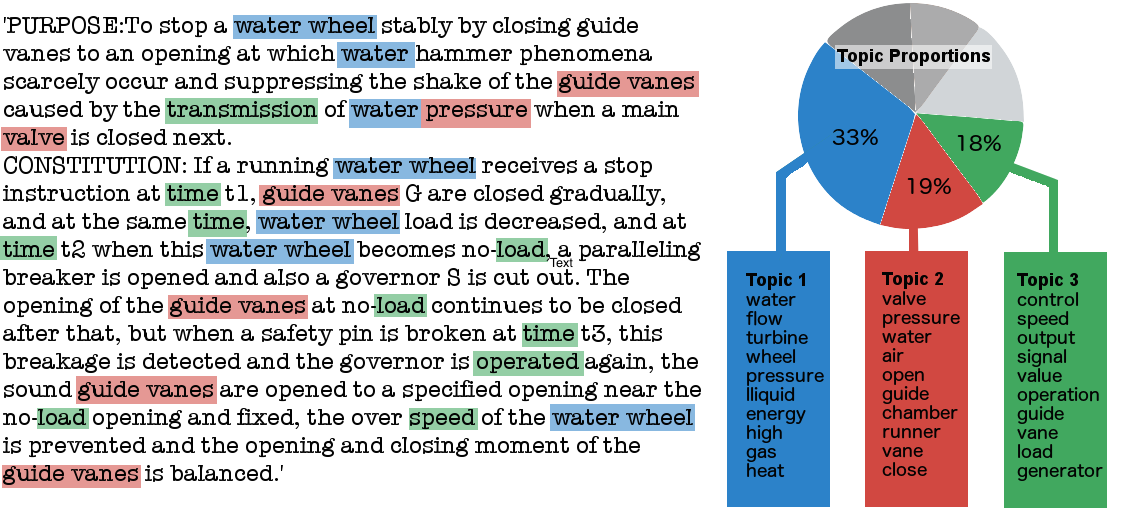
\includegraphics[width=130mm,scale=0.45]{Figures/Patent114}
\decoRule
\caption[Patent114]{Topic proportions in a sample patent abstract.}
\label{fig:Patent_114}
\end{figure}

The topics in the previous example were formed not over a single document but over a collection. The grey sections of the pie chart above represent the topics that this patent does not contain strong elements of. This is a key characteristic of LDA topic models, each document has a unique topic 'fingerprint' as a result of a generative process. That process for generating a document word by word is as follows. First we decide, sampling from the distribution of topics, which topic our first word will belong to. Then we sample from that chosen topic's distribution to decide what the word itself will be. This process is then simply repeated for each word, and while it works it has the following assumptions worth noting:

% assumptions
\begin{itemize}
\item Documents can manifest multiple topics (however typically not many)
\item Each document is assumed to be the product of a generative process.
\item Generative process starts with a topic, i.e. a distribution over a fixed vocabulary.
\item Assumes a fixed number of topics
\end{itemize}

% math framework.
Latent Dirichilet allocation falls into a family of machine learning algorithms called \keyword{hidden variable models}.  In this family of models, the user customarily "posits a hidden structure in the observed data, and then learns that structure using posterior probabilistic inference" \parencite{TopicModels2009}. For LDA specifically, the documents are the observed data, the topics and document topic proportions are hidden.

More formally, we may define this process mathematically as a joint distribution over our hidden variables and our observed variables. Specifically, we define the distribution over vocabulary as $\beta$, the topic proportions for document d $\theta_d$, the topic assignment for a word in a document $z_{d,n}$ and of course the observed words themselves $w_{d,n}$. 

\begin{align*}
  & P(\beta_{1:K},\theta_{1:D},z_{1:D},W_{1:D}) \nonumber \\
  & = \prod_{i=1}^K p(\beta_i) 
  \prod_{d=1}^D p(\theta_d)
  \{ \prod_{n=1}^N p(z_{d,n}|\theta_d)p(w_{d,n}|\beta_{1:k},z_{d,n}) \} \numberthis \label{eq:JointProb} 
\end{align*}

In Eq \ref{eq:JointProb} we see a few dependencies worth noting. Firstly that the topic we assign to a word $z_{d,n}$ depends on the distribution of topics of its document $\theta_d$. Additionally, that the identity of the word itself is dependent on not only the topic we assigned to generate it $z_{d,n}$, but also the vocabulary distributions of each topic $\beta_{1:K}$. Equivalently we can express the dependencies between these variables as a graphical model, illustrated in figure \ref{fig:Gmod1}.

\begin{figure}[ht]
\centering
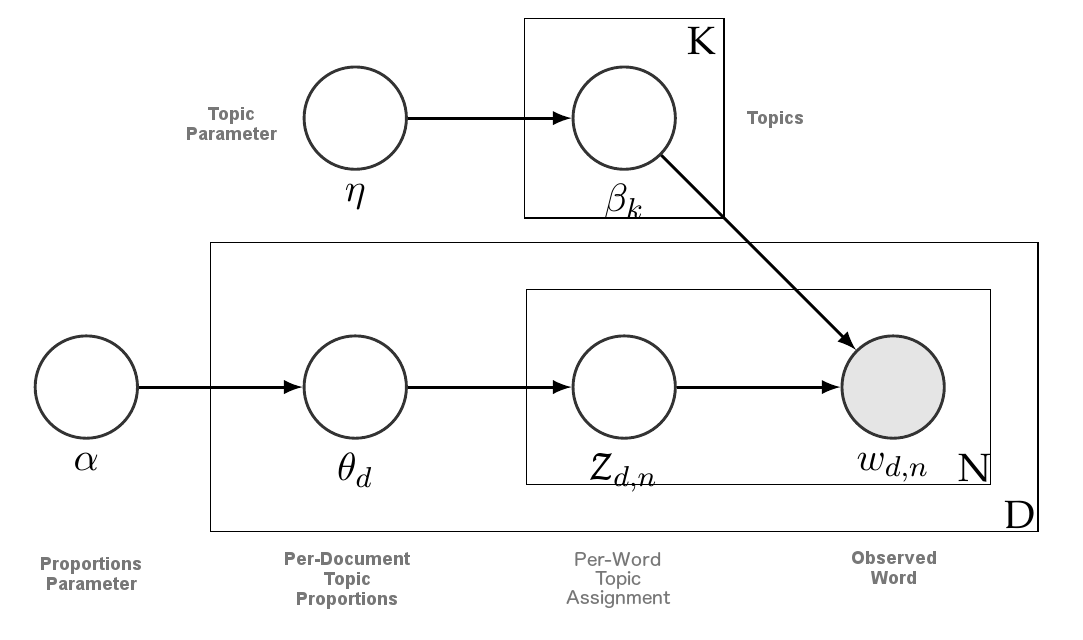
\includegraphics[width=130mm,scale=0.45]{Figures/gmod1}
%\begin{tikzpicture}
%\tikzstyle{main}=[circle, minimum size = 10mm, thick, draw =black!80, node distance = 16mm]
%\tikzstyle{connect}=[-latex, thick]
%\tikzstyle{box}=[rectangle, draw=black!100]
%  \node[main, fill = white!100] (alpha) [label=below:$\alpha$] { };
%  \node[main] (theta) [right=of alpha,label=below:$\theta_d$] { };
%  \node[main] (T) [right=of theta,label=below:$T_{d,n}$] {};
%  \node[main] (eta) [above=of theta,label=below:$\eta$] { };
%  \node[main, fill = black!10] (w) [right=of T,label=below:$w_{d,n}$] { };
%  \node[main] (beta) [above=of T,label=below:$\beta_k$] { }; 
%  \path (alpha) edge [connect] (theta)
 %       (theta) edge [connect] (T)
  %      (T) edge [connect] (w)
  %      (beta) edge [connect] (w)
  %      (eta) edge [connect] (beta);
%  \node[rectangle, inner sep=0mm, fit= (T) (w),label=below right:N, xshift=13mm] {};
%  \node[rectangle, inner sep=4.4mm,draw=black!100, fit= (T) (w)] {};
 
%  \node[rectangle, inner sep=4.6mm, fit= (theta) (T) (w),label=below right:D, xshift=26.0mm] {};
%  \node[rectangle, inner sep=9mm, draw=black!100, fit = (theta) (T) (w)] {};
  
%  \node[rectangle, inner sep=4.6mm, fit= (beta),label=above right:K, xshift=-5.0mm, yshift=-5.0mm] {};
%  \node[rectangle, inner sep=4.6mm, draw=black!100, fit = (beta)] {};
%\end{tikzpicture}
\caption{Graphical model for LDA}
\label{fig:Gmod1}
\end{figure}

So how do we actually obtain our estimates of the hidden parameters? We need to calculate the conditional distribution of our hidden parameters (the topic structure), and the observed words i.e. the posterior distribution described in Eq. \ref{eq:LDAPost}. However the denominator makes this calculation computationally infeasible due to the number of combinations our hidden parameters could take. 

\begin{align}
  p(\beta_{1:K},\theta_{1:D},Z_{1:D}|W_{1:D}) = \frac{p(\beta_{1:K},\theta_{1:D},Z_{1:D}|W_{1:D})}{p(W_{1:D})} \numberthis \label{eq:LDAPost}
\end{align}

To move past this, most solutions use either sampling or variational based methods to perform approximate inference and obtain estimates of the hidden parameters. Variational methods allow us to translate the original problem to one of optimization and take advantage of the many optimization techniques available. This in turn allows us to make extensions that are often faster, scale better or allow for different forms of input such as streaming documents. 


%----------------------------------------------------------------------------------------
\section{Adding a temporal component}
% how is the DTM different?
One such extension, and the extension we explore in this study, is to relax the implicit assumption of LDA that the order of the documents doesn't matter. 
By incorporating the order of the documents to the model, a topic is no longer simply a distribution over words but now becomes a \emph{sequence} of distributions over words. This is the jump that allows us not only to identify a theme, as with static LDA, but also track how it progresses in time, giving us the Dynamic Topic Model (\keyword{DTM}).

%this is friggin' cool and you should be interested because it allows us to do some awesome stuff.
% - describe how a dynamic model might improve on the "normal" LDA
% - describe the usefulness of having a temporal component in the model. (maybe give specific example documents)
The DTM offers several advantages over traditional LDA including improved predictive performance \parencite{Blei:2006:DTM:1143844.1143859}. Primarily though, it facilitates a greater understanding of how each topic developed, and how the ideas therein formed and matured. With it, we can inspect trends of word usage to uncover a richer and more detailed hidden structure. For instance figure \ref{fig:wwttTopic6} contains a sample theme from a sub-collection of hydroelectric patents and the progression of word prevalences within it over time.

% super quick example
\begin{figure}[ht]
\centering
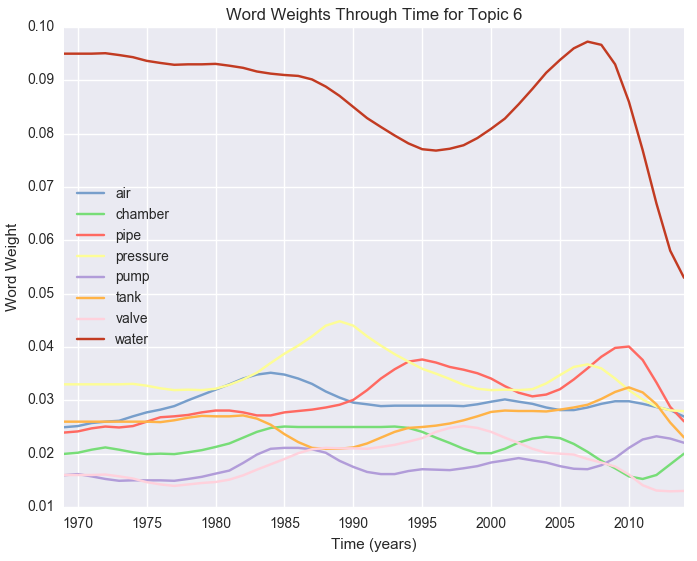
\includegraphics[width=130mm,scale=0.45]{Figures/wwttTopic6}
\decoRule
\caption[wwttTopic6]{Distribution over words in a sample hydroelectric topic over time}
\label{fig:wwttTopic6}
\end{figure}

%high level quick overview of the math? Or save it for the DTM section...
% DIDNT EVEN MENTION THE DIM!!!

%---modeling influence------
%\section{Modeling Influence}
% influence measurements of scientific journals and articles help determine decisions about funding and publishing. Traditionally this is done using citations (Garfield 2002) with the intuition that if more people cite a work, it is likely to be more influential.

% while scientific papers and in our case patents contain citations many texts don't such as news, blogs, legal documents.

% all citations are also counted equally as having contributed to a work which is rarely the case.

% new intuition that an influential paper will affect the language of subsequent related papers in a variable manner.

% DIM is the sibling of DTM



%----------------------------------------------------------------------------------------
\section{Why patents?}
% - reference why applying it to patents is not an accident. 
% i.e. why patents provide an interesting use case.
Patent data is specifically interesting in this context because of the role patents play in company formation, job growth, economic development, and novel invention. Their history tells a story of technological progression. In an attempt to maintain a competitive edge, many companies large and small spend a considerable amount of energy researching this history to identify technical trends relevant to their industry. 

% what's even more cool, is applying that DTM to patent data. we can effectively track the progression of innovation through language use in patent abstracts. 
Dynamic topic models have the potential to aid this research by enabling us to track the evolution of innovation through language use in patent abstracts. In this paper we look at a number of elements, including the evolution of technological themes and their proportions, the origination and development of language, as well as document influences. Furthermore, the patent corpus and associated International Patent Classification (\keyword{IPC}) labels provide a platform for the comparison of various topic modeling algorithms.

%research into new products or industries does not occur in a vacuum. 

%----------------------------------------------------------------------------------------
\section{Experiments}
% So, now that you know what LDA is, why it's important, what the DTM is and how we're applying it, here's what we tried out and what we were looking for.  Maybe give some intuition. (insufficiencies in previous methods of testing)

At the time of writing this, surprisingly little has been published exploring the effectiveness of both the DTM and the DIM. Much research has evaluated model quality solely based on the likelihood of held-out predictions, however likelihood does not always translate to semantically meaningful topics \parencite{Chang:Boyd-Graber:Wang:Gerrish:Blei-2009}. Additionally, the predictive performance of these models is adversely affected by longer time horizons due to an "increase in the rate of specialization in scientific language" \parencite{Blei:2006:DTM:1143844.1143859}. Acknowledging the room to explore alternative methods of model evaluation, we implemented the experiments listed below. 

\subsubsection{Historical Topic Trend Validation}
The simplest, but also the most hands-on, method of evaluating the quality of topics produced by the DTM and DIM is simply to validate the inferred topic trends against known industry history. For instance, if in the topic of water purification systems we observe a rise in the usage of words "2D materials" and "lattice membranes" around 2005, we might substantiate this by pointing out graphene's isolation the previous year in 2004.
 
% Figure XXX contains examples of patents matching historical technological trends.

\subsection{Topic Coherence}
In light of research suggesting that likelihoods and perplexity don't always correlate with human judgement on the interpretibility of topics \parencite{Blei:2006:DTM:1143844.1143859} we borrow several methods of topic coherence suggested by \parencite{DBLP:journals/corr/RosnerHRNB14}. Namely, we evaluated model topic coherences using C$\_$v, C$\_$npmi,C$\_$uci, and U$\_$mass. Using C$\_$v, the metric most correlated with human judgement, DTM achieved the highest with score with XXX compared to static LDA with YYY. For complete results see Table ZZZ in Section 5.


\subsection{Classification}
We wished to evaluate the proficiency of the word vectors unsupervisedly generated by the DTM and DIM at forming an effective feature space for document categorization. To do this we made use of the IPC labels of patents as broad class labels for text content. The resulting topic vectors should then help identify which class a document belongs to. Naturally we tested the efficacy of each model's vector space at correctly classifying the IPC label of documents when fed to a range of classification algorithms. Peak classification performance of the DTM based classifiers was F1 XXX, while LDA was F1 YYY. Text classification results are given in section ZZZ.
%DTM outperformed LDA by an average of XXX percent. Results in Table YYY.

%text categorization
%semantic evaluation
%evaluation measure for word vectors
%embeddings of texts

%Whether the resulting document vectors were useful for document classification


\subsection{Clustering}
Another method we used to evaluate the quality of the resulting document vectors was by their ability to cluster the documents. In order to determine which models yielded vector spaces of the corpus that most effectively defined separations in the data relative to the ground truth CPC labels we used the following metrics: the adjusted rand index, normalized mutual score info, homogeneity, completeness and the V-measure which we cover in section \ref{litreview}. Indeed we found that the DTM's vector space tended to outperform that of LDA at clustering with a peak NMI score of XXX compared to YYY. For more detailed results, refer to table ZZZ in section 5. 


%\subsection{Influence Estimation}
%Usefulness as a measure of influence (f. citations and pagerank) 
% typical patent analysis usually includes forward citations as a measure of patent 'value' either economically or technologically.
 

% - If you believe all of these things you should give me a distinction. If not, read on...

\section{Roadmap of Paper}
% roadmap
The overall structure of this paper is as follows. In \textbf{chapter \ref{Chapter2}} we review the literature surrounding the applications and various evaluation methods for topic models,  and also give a detailed account of both the DTM and DIM.
Then in \textbf{Chapter \ref{Chapter3}} we cover the experimental set up and considerations in data preparation. The results of our experiments are subsequently presented in \textbf{Chapter \ref{Chapter4}}, and finally we conclude in \textbf{Chapter \ref{Chapter5}} with a discussion of results and suggestions for future study.

%----------------------------------------------------------------------------------------

%qualitative exploratory tasks and quantitative predictive and classification tasks.



%% Chapter 2
\chapter{Background Information and Theory} 
\label{Chapter2} 


%----------------------------------------------------------------------------------------
\section{Literature Review} \label{litreview}
% literature review is a paper or article you might sit down to read that gives a general overview of a field. someone not experienced in topic modelling should come a way with a greater understanding of topic models after reading it. And be ready to understand more of your project. 
% explain here what we are going to cover in the literature review.

In this section we begin by reviewing a few of the tasks common in topic modeling. Then we describe a handful of the ways the quality of topic models, LDA in particular, are commonly tested. Finally we discuss the specific tasks of document classification and clustering in the context of topic modeling, as well as the corresponding methods for evaluating model performance at these tasks. 

\subsection{Applications of Topic Modeling}
%------General---------
The most popular application of topic models is simply summarizing large text collections by mining the topics. This is a task LDA is particularly suited for \parencite{griffiths_steyvers04, Mei:2007:ALM:1281192.1281246}. The original LDA paper however \parencite{Blei:2003:LDA:944919.944937} gave promising results on document classification as well. Since then LDA has been used with success not only for document classification, but also for clustering and information retrieval \parencite{Wei:2006:LDM:1148170.1148204, Nagwani2015}. This is due to the strength of the topic vectors LDA models provide, which tend to correlate strongly with human judgement. 

%Though significantly less work has been done assessing the efficacy of LDA extensions such as the DTM and DIM in these areas. 

\subsection{Ensuring Model Quality}
%------Methods of Testing------
\subsubsection{Perplexity Testing}
In order to ensure the strength of these topic vectors researchers employ a handful methods to evaluate the topic models. While the most intuitive method is simply to have humans judge the coherence of each topic, this becomes prohibitively time consuming and expensive for large data sets. One commonly used method of automating this process is by evaluating the topic model on a held out set of testing documents and obtaining the log-likelihood perplexity of the unseen documents \parencite{Blei:2003:LDA:944919.944937, wallach-murray-rsalakhu-mimno-2009}. A higher likelihood on unseen documents, and a lower perplexity score indicates a better model. However this method of evaluating topic model performance has several issues. Firstly, it has been shown that predictive likelihood, or equivalently perplexity, is not always correlated with human judgement, and in some cases is even slightly anti correlated \parencite{Chang:Boyd-Graber:Wang:Gerrish:Blei-2009}. Secondly this method of evaluation only acts as a general measure of the entire model. What about the quality of the individual topics?


% Prior testing of the DTM and DIM specifically, is also based on held out likelihood or perplexity, which as we've mentioned doesn't always correlate with human judgements \parencite{Chang:Boyd-Graber:Wang:Gerrish:Blei-2009}. This leaves considerable room for the exploration and evaluation of both the DTM and DIM on the aforementioned tasks of document classification and clustering.

%DIM involves correlating influences with citation, we replicate and extend by adding page rank

\subsubsection{Coherence Testing}
%------Coherence Testing--------
%why are we not using tfidf?
Fortunately several methods of evaluating the coherence of individual topics from topic models exist. For a topic $t$ we define the \keyword{Umass} coherence as a sum of the pairwise scores of that topic's top words  $W_t =  \{w1, ... w_n\}$. 

\begin{align*}
\text{Umass Coherence } c(t,W_t) &= \sum_{w_i,w_j \in W_t} \text{score}(w_i,w_j) \\
&= \sum_{w_i,w_j \in W_t} log \frac{d(w_i,w_j) + \epsilon}{d(w_i)}
 \numberthis \label{eq:coherence} 
\end{align*}

Where $d(w_i)$ is the number of documents containing the word $w_i$ and $d(w_i,w_j)$ is the number of documents containing both word $w_i$ and $w_j$. The $\epsilon$ in the numerator is simply to smooth the counts and is typically set to a minimal value such as 1 or .01. Intuitively then, a topic is good if its words cooccur often \parencite{Mimno:2011:OSC:2145432.2145462}.

The \keyword{UCI} measure introduced by \parencite{NewmanBB11}, operates in the same manner as Umass but with the pointwise mutual information as a scoring function instead, given in eq \ref{eq:uci}.

\begin{align*}
\text{UCI Coherence } = c(t,W_t) &= \sum_{w_i,w_j \in W_t} \text{score}(w_i,w_j) \\
&= \sum_{w_1,w_2 \in W_t} log \frac{p(w_i,w_j)}{p(w_i)p(w_j)}
 \numberthis \label{eq:uci} 
\end{align*}

Where $p(w_i)$ is the probability of seeing word $w_i$ in a random document and $p(w_i,w_j)$ is the probability of seeing both word $w_i$ and word $w_j$ together in a random document. It should be noted that obtaining these probabilities requires empirically estimating them from an external dataset. 

Two more noteworthy measures of topic coherence, in addition to those outlined above, were developed by Roder, Both and Hinneberg in their study titled "Exploring the Space of Topic Coherence Measures" \parencite{Roder:2015:EST:2684822.2685324}. These measures were the  \keyword{C$\_$v} and \keyword{C$\_$npmi} measures which demonstrated a substantial correlation with human judgement. For brevity we do not replicate their derivations here, but the interested reader will find a detailed description of each in \parencite{Roder:2015:EST:2684822.2685324}

%In a series of experiments on on word sets generated form English and German Wikipedia articles, one study found that a baseline "one-vs-all" approach often outperformed the Umass coherence measure \parencite{DBLP:journals/corr/RosnerHRNB14}.


\subsection{Document Classification}
\label{classificationmetrics}
%------Text Classification---------
Though the topics produced by topic models are useful in their own right for the qualitative analysis of documents, they are also useful quantitatively when trying to classify documents. For instance a large news organization may want to automatically sort its thousands of articles into the categories "politics", "natural disasters" and "sports". To do this they might use a topic model to get a vector of topic proportions for each document to use as features for a classification algorithm. This process is referred to as document vectorization.

% could use tfidf but LDA is sometimes better
While baseline methods for document vectorization exist, such as the Term Frequency Inverse Document Frequency (tf-idf), LDA has been shown to outperform them in certain scenarios. For instance when less training data is available LDA boasted a shorter training time and higher classification accuracy  \parencite{liempirical}. Additionally when tested against other baseline methods for document vectorization such as the unigram model or probabilistic latent semantic analysis (PLSA), LDA again proved consistenlty more accurate at document classification tasks \parencite{Lu:2011:ITP:1969504.1969510}. 

\subsubsection{Accuracy}
When it comes time to evaluate a model's classification performance there are several approaches, the most intuitive of which is accuracy. Accuracy is defined as  

\begin{align*}
acc = \frac{Tp + Tn}{Tp + Tn +Fp + Fn}
 \numberthis \label{eq:acc} 
\end{align*}

Where $Tp$ are our true positives, $Tn$ are our true negatives, $Fp$ are our false positives, and $Fn$ are our false negatives. It should be noted that normal values of accuracy for classification tasks depend highly on the data at hand. Noisy data or a large number of classes can both artificially drive accuracy scores down. 

\subsubsection{Precision}
But what if we want to know, out of the total number of guesses for a particular class, what fraction were correct? For this, researchers typically use the Precision, defined as

\begin{align*}
p = \frac{Tp}{Tp + Fp}
 \numberthis \label{eq:precision} 
\end{align*}

\subsubsection{Recall}
Conversely, if we wish to know out of the total number of cases we could have guessed correctly, what fraction we \emph{did} guess correctly then Recall is typically used. Recall is defined as

\begin{align*}
r = \frac{Tp}{Tp + Fn}
 \numberthis \label{eq:recall} 
\end{align*}

\subsubsection{F1 Score}
The F1 score is a way of combining the above two metrics Precision and Recall into one wholistic measure. Conceptually it is the harmonic mean of the Precision and Recall where we assign even weights to each. The F1 score is defined as


\begin{align*}
F_1 &= \frac{1}{\frac{1}{2}\big( \frac{1}{p} + \frac{1}{r}} \\
&= \frac{2pr}{p+r}
 \numberthis \label{eq:f1} 
\end{align*}

%Again though, prior work indicates no testing of either DTM or DIM in this regard, both of which offer improvements in the latent semantic representation of ordered document collections.

\subsection{Document Clustering}
\label{DocumentClustering}
%------Clustering-------
Another well established task for topic models is document clustering. LDA has been used to successfully cluster a range of documents such as news articles and legal judgements \parencite{Lu:2011:ITP:1969504.1969510, DBLP:journals/corr/XieX13, Kumar2013}. As opposed to classification where we want to assign an explicit label to each document, with clustering we wish to evaluate how well the resulting document topic vectors separate the documents into a meaningful structure.

\subsubsection{Adjusted Rand Score}
One way of accomplishing this is by using the \keyword{Adjusted Rand Score} which measures the similarity of two sets of class labels; namely the true labels $C$ and those predicted by a clustering algorithm $K$. We may calculate the raw (unadjusted) Rand index following equation \ref{eq:RI} \parencite{Hubert1985}. 

\begin{align*}
RI = \frac{a + b}{C_2^{n_{\text{samples}}}}
 \numberthis \label{eq:RI} 
\end{align*}

Where $a$ is the number of pairs of elements in $C$ belonging to the same class, and in $K$ belonging to the same class. Conversely $b$ is the number of pairs of elements in $C$ belonging to different classes, and in $k$ belonging to different classes. Finally, $C_2^{n_{\text{samples}}}$ is the total number of possible pairs in the dataset. In order to ensure that random labelings receive a score of zero we define the adjusted Rand index as 

\begin{align*}
ARI = \frac{RI - E[RI]}{max(RI) - E[RI]}
 \numberthis \label{eq:ARI} 
\end{align*}

\subsubsection{Normalized Mutual Info}
The Normalized Mutual Info is another method of evaluating clustering performance that has been successfully applied in the context of topic modelling \parencite{Xu:2003:DCB:860435.860485, Cai:2008:MHT:1458082.1458202}. It again assumes we have two sets of labels, this time we call them $U$ and $V$, over $N$ objects. We define the entropy of a label set $U$ in equation \ref{eq:entropy}, where $P(i) = |U_i|/N$ is the probability that a random object from $U$ falls into class $U_i$.

\begin{align*}
H(U) = \sum_{i=1}^{|U|} P(i)log(P(i))
 \numberthis \label{eq:entropy} 
\end{align*}

The mutual information (MI) between $U$ and $V$ can be expressed as 

\begin{align*}
MI(U,V) = \sum_{i=1}^{|U|} \sum_{j=1}^{|V|} P(i,j)log(\frac{P(i,j)}{P(i)P(j)})
 \numberthis \label{eq:MI} 
\end{align*}

With these two components we can write the normalized mutual information as proposed in \parencite{Vinh:2009:ITM:1553374.1553511}.

\begin{align*}
NMI(U,V) = \frac{MI(U,V)}{\sqrt{H(U)H(V)}}
 \numberthis \label{eq:NMI} 
\end{align*}

%\subsubsection{Homogeneity, Completeness and V-measure}


%----------------------------------------------------------------------------------------
\section{DTM Model Overview}

% Roadmap + Disclaimer
This section briefly outlines the dynamic topic model (\keyword{DTM}), following closely the original derivation found in \parencite{Blei:2006:DTM:1143844.1143859}. As this is intended as more of a summary, we recommend the reader examine the original paper for a complete exposition of the mechanics of the DTM. 

% Intuition + Conceptual Basis
In our primer on LDA (in section \ref{ldaprimer}) we outlined the conceptual basis for static LDA topic models. Namely, that topics consist of a distribution over a fixed vocabulary and are determined by a set of hyper-parameters $\beta$. Additionally each document is represented as a combination of topics, with proportions controlled by their corresponding set of hyper-parameters $\alpha$. Roughly speaking, the goal of the Dynamic Topic Model (\keyword{DTM}) is to account for the drift in topics over time by chaining together a series of static LDA models. This is accomplished by tying the hyper-parameters $\alpha_{t-1}, \beta_{t-1}$ at time step $t-1$, to the hyper-parameters $\alpha_{t}, \beta_t$ at time step $t$. The result is a model that allows us to track how our topics evolve at each time step. 


%The general approach is to chain together the underlying topic multinomials and topic proportion distributions, then to make use of the Kalman filter to carry out approximate posterior inference over the latent topics.

% how do we actually tie these hyper parameters together?
%With regular latent dirichilet allocation we normally use a Dirichilet distribution to model our uncertainties in word distributions, hence the name. However, this is no longer an option as the Dirichilet distribution does not permit sequential modeling. 

\subsection{Chaining models together}

The question then, is how do we tie our hyper-parameters together? Well, regularly with static LDA we would simply use a Dirichilet distribution to model our uncertainties in word distributions (hence the name). Unfortunately, the Dirichilet distribution does not lend itself to sequential modeling, which eliminates this option. Instead, we make a state-space model that evolves with Gaussian noise to chain together the natural parameters of each topic $\beta_{z,t}$ such that each topic "evolves" from the last.

\begin{align*}
\beta_{z,t} | \beta_{z,t-1} \sim  \mathcal{N}(\beta_{t-1,z},\sigma^2I)  \numberthis \label{eq:topicwordschain} 
\end{align*}

Similarly, with static LDA we would also pull our document specific topic proportions $\theta$ from the Dirichilet distribution. For the same reason as above this is no longer an option. So to express our uncertainty over our topic proportions, we use a logistic normal with mean $\alpha$. Then we chain our topic proportions together using the same trick as we did above with word distributions, (by using Gaussian noise). This yields the graphical model in figure \ref{fig:DTMGM}.

\begin{align*}
\alpha_{t} | \alpha_{t-1} \sim  \mathcal{N}(\alpha_{t-1},\delta^2I)  \numberthis \label{eq:topicpropschain} 
\end{align*}

\begin{figure}[ht]
\centering
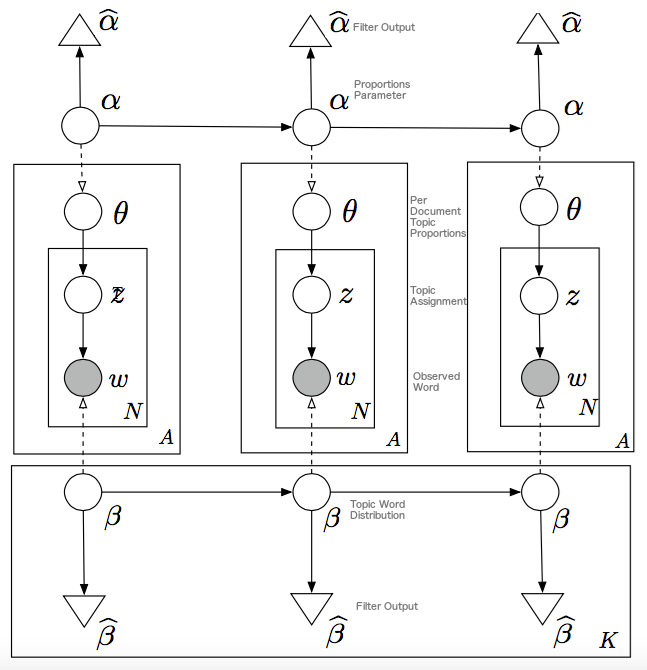
\includegraphics[width=130mm,scale=0.45]{Figures/DTMGM}
\caption[DTMGM]{Graphical model for DTM showing a series of chained static LDA models. The triangles represent the Kalman filter estimates of the hyper-parameters}
\label{fig:DTMGM}
\end{figure}

% could put in the new process from Blei here but maybe that's a bit too much like plagiarism? Would not be cool. 

\subsection{Variational approximate inference}
% motivating variational methods
Because we have used the Gaussian distribution to model the progression of our parameters, inference becomes intractable due to the non-conjugacy of Gaussian and multinomial models. To get around this we take the same variational approach to approximate inference as before in section \ref{ldaprimer} with static LDA. Taking a variational approach has the advantage of allowing us to handle larger document sets compared to Gibbs sampling which becomes computationally difficult at large corpus sizes. 

% variational methods
The general strategy of variational approximate inference is to use a carefully tuned 'approximate' distribution as a substitute for the true posterior. To tune this approximate distribution we minimize the KL divergence between our estimated and true posterior. Finally we may then use this approximated posterior distribution to perform inference.

We begin by creating a collection of variational parameters we will optimize over our latent variables. Our latent variables are the topics $\beta_{t,k}$, topic proportions $\theta_{t,d}$, and topic indicators $Z_{t,d,n}$. While we have variational parameters for each topic (consisting of a sequence of multinomial parameters), and for each document (the latent topic proportions). The resulting posterior, again following the notation of \parencite{Blei:2006:DTM:1143844.1143859} is given by equation \ref{eq:dtmpost}.

\begin{align*}
& \prod_{k=1}^K q(\beta_{k,1}, ... , \beta_{k,T} | \hat{\beta}_{k,1}, ... , \hat{\beta}_{k,T})  \times     \\
& \prod_{t=1}^T \Big( \prod_{d=1}^{D_t} q(\theta_{t,d})| \gamma_{t,d}) \prod_{n=1}^{N_{t,d}}q(z_{t,d,n}|\phi_{t,d,n})   \Big)  \numberthis \label{eq:dtmpost} 
\end{align*}

This is where we tune our approximate posterior, and specifically the variational observations $\{ \hat{\beta}_{k,1}, ... , \hat{\beta}_{k,T}  \}$ according to the KL divergence between the estimated and the true posterior. Note that here, each topic proportions vector $\gamma_{t,d}$ receives a corresponding free Dirichilet parameter, while each topic indicator $z_{t,d,n}$ receives a corresponding free multinomial parameter $\phi_{t,d,n}$. To optimize the document topic proportion vectors we subsequently employ gradient ascent, however this is not necessary for the document level parameter updates as they simply have a closed form.

%topic tracking
Finally, we may track our variational parameters $\hat{\beta}$ and $\hat{\alpha}$  between time slices using either the Kalman filter or wavelet regression. For brevity we will not replicate the mechanics of these methods here and encourage the interested reader to refer to the derivations provided in detail in  \parencite{Blei:2006:DTM:1143844.1143859}.


%\subsection{Issues}
%The DTM is not without its fallbacks. 
%addresses several latent structures in the document collection such as topic evolution and prevalence, however does not address the birth and death of topics, like models such as \cite{DBLP:journals/corr/abs-1203-3463}.

%--------------------------------------------------------------------------------------
%\section{DIM Model Overview} 

%language based approach to modeling the influence of documents.
%useful when traditional bibliometrics such as citations are not available. produces an internal measure of document influence that has been shown to correlate with citations. Closely related to the DTM but with XXX.

% important for decisions about publishing and funding
% also relevant to know for scientists who should read important work in their field for good research practice

%probability of a word given the natural parameters of the word distribution beta at time t

%then we have as in the DTM a logistic normal markov chain
%(its drift is a stationary autoregressive process)

%central idea: some articles influence the topic more than others.

%initialize normally distributed scalar influence scores $l_d$ to describe the influence article $d$ has on the topic. Higher influences mean a document had a larger affect on the drift of the topic.


%give equation of time series model


%word from documents of high influence will have a higher probability in the following time step while words from an article with zero influence will not affect the next time step. As with the dtm, once trained on our corpus the posterior of topic and influence scores gives gives a trajectory of term fre- quencies and a retrospective estimate of the influence of each article. An article whose words can help explain the way the word frequencies change will have a high posterior influence score

%[image of the graphical model]























 
%% Chapter 3

\chapter{Experimental Set Up} % Main chapter title

\label{Chapter3} % For referencing the chapter elsewhere, use \ref{Chapter3} 
In the interest of reproducibility we include in this section some of the considerations specific to our data set. Additionally we cover the data pre-processing steps taken prior to our experiments and describe our process for model tuning. Finally, we outline the procedure taken for the coherence testing, classification and clustering experiments. 

%----------------------------------------------------------------------------------------
\section{Data Considerations}

% THE DATASET
The data we used for our experiments comes from the August 2015 EPO Worldwide Patent Statistical Database (\keyword{PATSTAT}). According to the EPO, this data set contains over 90 million patent documents from leading industrialized and developing countries, with some documents as early as the nineteenth century. Thankfully, the expanse of this data is met with an equal level of documentation\footnote{For more information the official catalogue can be found at \url{http://goo.gl/LRQWnu}}. 


% CPC/IPC CLASSES
Due to time and computation limits, we ran experiments only on a subset of this data rather than the whole corpus. In order to break the PATSTAT into manageably sized subclasses we made use of Cooperative Patent Classification (\keyword{CPC}) labels. The CPC labels are a hierarchical system used globally to annotate patents according to the area of technology to which they relate. Predominantly we carried out our research on patents under the umbrella of \keyword{Y02E 10/20}, the subclass of patents relating to \keyword{hydro energy}. This subclass itself consisted of 5 smaller subsets of documents with more specific labels which we treated as true labels during our classification experiment, namely "Hydro energy", "Conventional", "Turbines and wheel", "Other parts", and "Stream and damless".

% PATENT FAMILIES
An additional consideration in filtering our data was the International Patent Documentation Centre \keyword{(INPADOC) patent family}. A patent family is a collection of patents filed in various countries to protect the same invention. We ensure that only one member of each patent family participates in the study so as not to 'double count' the same invention. Furthermore, only patents filed in English are considered. Figure \ref{fig:psqlSchema} contains the schema for the PostgreSQL database we constructed to hold relevant patent data.


\begin{figure}[h]
\centering
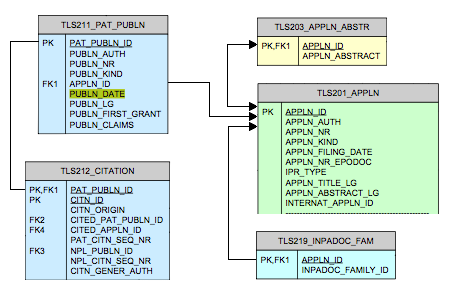
\includegraphics[width=130mm,scale=0.45]{Figures/psql_schema}
\decoRule
\caption[PSQLSchema]{Schema of PostgreSQL database containing relevant tables}
\label{fig:psqlSchema}
\end{figure}

% FORWARD CITATIONS
% how were forward citations calculated

% include  of subsetdatabase schema?
% stored in psql

\section{Data Pre-Processing}

%stopping, stemming, lower case, min_freq
The phrase "garbage in garbage out" is commonly used in machine learning to emphasize the importance of the data pre-processing step. We begin our pre-processing by retrieving abstracts from the aforementioned PSQL database and applying case folding such that words like "Turbine" at the beginning of a sentence will match the word "turbine" elsewhere. We then remove unnecessary symbols and punctuation via regex and apply stopping using the English \keyword{NLTK} stopwords list. This effectively removes common conjunctions and operational words from our corpus that don't actually contribute to the topics, such as "but, if, the, and" etc. 

\begin{tikzpicture}[node distance=4mm, >=latex',
 block/.style = {draw, rectangle, minimum height=10mm, minimum width=28mm,align=center},
rblock/.style = {draw, rectangle, rounded corners=0.5em},
tblock/.style = {draw, trapezium, minimum height=10mm, 
                 trapezium left angle=75, trapezium right angle=105, align=center},
                        ]
    \node [rblock]                   (a)     {Retrieve abstracts from PSQL};
    \node [block, right=of a]    (b)   {Tokenization, \\
	Regex cleaning $\&$ \\    
    Casefolding
    };
    \node [block, right=of b]   (c)  {Stopping};
    \node [block, below=1.2cm of a]  (d)      {Lemmatization};
    \node [block, right=of d]  (e)  {Frequency\\ Filtering};
    \node [tblock, right=of e]  (f)     {Serialize\\
    $\&$\\ Save};
    \node [coordinate, below right =.5cm and .5cm of c] (right) {}; 
    \node [coordinate, above left =.5cm and .5cm of d] (left) {}; 
    
    \path[draw,->] (a)      edge (b)
							 (b)      edge (c)
							 (c.east) -| (right) -- (left) |- (d)
							 (d)      edge (e)
							 (e)      edge (f)                    
                    ;
    \end{tikzpicture}

We then further distill the abstracts by applying lemmatization. This step is meant to reduce inflectional forms of a word such as "operates, operating, operational" to a base form "operate". After lemmatization, we remove any words occurring less than 25 times total, matching the implementation found in \parencite{Blei:2006:DTM:1143844.1143859}. Finally, we save the resulting corpus, totaling over 6,400 documents, and serialize the dictionary of vocabulary for subsequent access.

% number of unique words?

% used gensim, Python, Postgresql, ipython notebooks

\section{Tuning models}
\label{tuning}
The hyperparameters we select for our models can have a large influence on the topics that they infer. For this reason, prior to running any experiments, it is important to tune the hyperparameters of our topic models. The parameters we tuned specifically, were the number of topics $K$ and the maximum number of iterations $M_{iter}$. To do this we defined a range of values for these parameters and sampled parameter sets from this space uniformly. At each parameter set we evaluated the \keyword{umass}, \keyword{uci}, \keyword{npmi}, and \keyword{cv} topic coherence of the resulting model. 

In order to inspect the relationship our parameters had with topic coherence we visualized our results. Figure \ref{fig:DTMUCI} displays the c$\_$uci coherences of the DTM as a function of $K$ and $M_{iter}$. From this plot we can see that increasing the number of topics $K$ beyond a certain point fails to improve topic coherence with similar results for the number of iterations.

\begin{figure}[h]
\centering
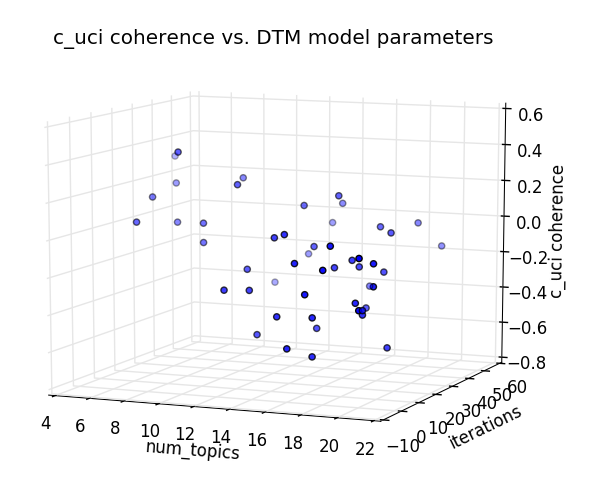
\includegraphics[width=130mm,scale=0.45]{Figures/uciCoherence}
\decoRule
\caption[DTMUCI]{c$\_$uci coherence scores for the DTM as a function of $K$ and $M_{iter}$}
\label{fig:DTMUCI}
\end{figure}

Table \ref{tab:paramtune} contains the best coherence scores obtained by each model for each measure after sampling our constrained parameter space. Despite tuning the models on a smaller set of documents it is interesting to note that a trend emerges, namely that the DTM tends to outperform both the DIM and the static LDA model in terms of topic coherence. However we reserve judgement until obtaining the final coherence testing results listed in section XXX. 

\begin{table}[ht]
\caption[HParamTuning]{The peak coherences achieved for various models and parameter choices.}
\label{tab:paramtune}
\centering
\begin{tabular}{l l l l l}
\toprule
\tabhead{Model} & \tabhead{c$\_$v} & \tabhead{c$\_$uci} & \tabhead{c$\_$npmi} & \tabhead{u$\_$mass} \\
\midrule
LDA & .4871 & .1455 & .0694 & -0.9813 \\
DTM & .5999 & .4098 & .1287 & -1.4496 \\ %.5916
DIM & .5789 & .1145 & .1175 & -1.6033 \\
\bottomrule\\
\end{tabular}
\end{table}

Though the optimal parameter sets suggested by each coherence measure did not greatly differ from one another, ultimately we selected the parameters recommended by the c$\_$v measure. We preferred the judgement of the c$\_$v measure as it is known to have the strongest correlation with human judgement \parencite{Roder:2015:EST:2684822.2685324}. The optimal parameter set found for the LDA model under the c$\_$v measure was $K$ = 13, $M_{iter}$ = 40, while for the DIM it was $K$ = 5, $M_{iter}$ = 32, and for the DTM it was $K$ = 17, $M_{iter}$ = 36. These were the parameters we used for the full scale coherence testing reported in section XXX.


%setting the alpha parameter in LDA as recommended by (e.g., as in Steyvers and Griffiths 2007) It acts as a form of regularization.
%A recommended setting is a = 50/K (Griffiths and Steyvers 2004; Steyvers and Griffiths 2007)

\section{Experimental Procedures}

\subsection{Coherence Testing}
% how we tested coherences of the models
The coherence testing experiment follows much the same procedure as above for hyperparameter tuning, with the difference being a full data set, and defined model parameters. We begin by training the LDA model, DTM and DIM over the same set of input documents belonging to the \keyword{Y02E 10/20} hydro energy CPC label, ranging from the year 1997 to 2015. Each model was trained under the optimal parameters found via the hyperparameter tuning process from section \ref{tuning}. 

Following model training, we retrieved all topics from the LDA model, DTM and the DIM, and assessed their semantic value via the \keyword{c$\_$v}, \keyword{c$\_$uci}, \keyword{c$\_$npmi}, and \keyword{U$\_$mass} coherence metrics. However because the DTM and DIM both output a \emph{series} of topics rather than a single set, the topic coherences were tested at each time step. Results for this experiment can be found in section XXX.

\subsection{Classification}
% how we classified 
To asses the efficacy of each model at creating feature vectors useful for document classification we begin by taking the same models as above, (the LDA model, DTM and DIM, trained on the hydro electric patents) and extract the document topic vectors for each document.

We then use 80$\%$ of these unsupervisedly learned feature vectors to train a collection of classifiers, and tested on the remaining 20$\%$ using the CPC subclasses for each document as true labels. We cross validated each classifier to ensure more robust estimates of performance, and selected the results of the classifier with the highest cross validated F1 score for each topic model. To further analyze the performance of each topic model's peak classifier we made use of the classification metrics outlined in section \ref{classificationmetrics} namely \keyword{accuracy}, \keyword{precision}, \keyword{recall}, and \keyword{F1 score}. Results for this experiment can be found in section XXX.


\subsection{Clustering}
% how we carried out clustering
Lastly, we conduct a clustering experiment to determine how well each model creates internally consistent groups of documents that are distinct from one another. We begin with the same set of models and data as with the other experiments, namely the LDA model, DTM and DIM trained on hydro electric PATSTAT patents. As with the classification experiment, we again extract the document topic vectors for each document.

However for this experiment, rather than beginning by handing the vectors to a series of classifiers, we begin by visualizing the space they formed using \keyword{TSNE}, \keyword{PCA}, and \keyword{MDS} embeddings to inspect the clusters by eye. After visually inspecting each model's document vectors we performed K-means clustering with $K=5$, (the number of true topics in the corpus). To evaluate clustering performance we feed the labels estimated by K-means for each set of document vectors, (alongside the respective true labels), to each of the clustering metrics outlined in section \ref{DocumentClustering}. These metrics include the \keyword{adjusted rand score}, \keyword{normalized mutual info}, \keyword{homogeneity}, \keyword{completeness} and \keyword{V-measure}. Results for this experiment can be found in section XXX.


%% Chapter 4

\chapter{DTM Results and Insights} % Main chapter title

\label{Chapter4} % For referencing the chapter elsewhere, use \ref{Chapter4} 

%----------------------------------------------------------------------------------------


%----------------------------------------------------------------------------------------
\section{Topics Through Time}

\subsection{validating topic histories in technology}



 
%% Chapter 5

\chapter{DIM Results and Insights} % Main chapter title

\label{Chapter5} % For referencing the chapter elsewhere, use \ref{Chapter5} 



%----------------------------------------------------------------------------------------
\section{Influence Metric}

\subsection{validating influential patents}

\subsection{correlation with forward citations}

\subsection{correlation with page-rank}



 

%----------------------------------------------------------------------------------------
%	THESIS CONTENT - APPENDICES
%----------------------------------------------------------------------------------------

\appendix % Cue to tell LaTeX that the following "chapters" are Appendices

% Include the appendices of the thesis as separate files from the Appendices folder
% Uncomment the lines as you write the Appendices

% Appendix A

\chapter{Appendix Title Here} % Main appendix title

\label{AppendixA} % For referencing this appendix elsewhere, use \ref{AppendixA}

Write your Appendix content here.
%\include{Appendices/AppendixB}
%\include{Appendices/AppendixC}

%----------------------------------------------------------------------------------------
%	BIBLIOGRAPHY
%----------------------------------------------------------------------------------------
%EPO Worldwide Patent Statistical Database August 2014
\printbibliography[heading=bibintoc]

%----------------------------------------------------------------------------------------

\end{document}  
